% Shared preamble for the three worksheets (compile with xelatex).
\documentclass[12pt]{article}
\usepackage[letterpaper,left=0.5in,right=0.5in,top=0.4in,bottom=0.4in,includefoot=false,nohead]{geometry}
\usepackage{fontspec}
\setmainfont{Andika}
\usepackage{xcolor}
\usepackage{tikz}
\usetikzlibrary{arrows.meta,calc}
\usepackage{array}
\usepackage{enumitem}
\usepackage[most]{tcolorbox}
\setlist{nosep,leftmargin=1.4em}
\pagestyle{empty}
\setlength{\parindent}{0pt}
\setlength{\parskip}{0pt}
\hyphenpenalty=10000 \exhyphenpenalty=10000 \sloppy
\makeatletter\g@addto@macro\@parboxrestore{\raggedright}\makeatother
\AtBeginDocument{\raggedright}

% ---- pattern block colours ----
\definecolor{pbgreen}{HTML}{2E9E48}
\definecolor{pbblue}{HTML}{2160C4}
\definecolor{pbred}{HTML}{D7302F}
\definecolor{pbyellow}{HTML}{F2C318}
\definecolor{pbpurple}{HTML}{7B3FA0}
\definecolor{ribbontext}{HTML}{A3201C}
\definecolor{ribbontextB}{HTML}{1E6B32}
\definecolor{inkgray}{HTML}{555555}

\tikzset{
  gridline/.style={line width=0.5pt,draw=black!32},
  dotgrid/.style={line width=0.9pt,draw=black!35,dash pattern=on 1.2pt off 3pt},
  boardline/.style={line width=1.8pt,draw=black},
  holefill/.style={fill=black!78},
  upfill/.style={fill=black!20},
  recgrid/.style={line width=0.35pt,draw=black!28},
  recline/.style={line width=1pt,draw=black!85},
  tileedge/.style={line width=0.9pt,draw=black!85},
  tileoutline/.style={line width=1.5pt,draw=black},
  hlfill/.style={fill=pbyellow!60},
  ribbonfill/.style={fill=pbred!28},
  ribbonfillB/.style={fill=pbgreen!35},
  ribbon arrow/.style={-{Stealth[length=5pt]},line width=1.3pt,draw=ribbontext},
  flip arrow/.style={{Stealth[length=6pt]}-{Stealth[length=6pt]},line width=1.2pt},
  piece/.style={line width=0.8pt},
  iconline/.style={line width=0.5pt,draw=black!80},
  cubeL/.style={fill=black!62},
  cubeR/.style={fill=black!22},
  cubeS/.style={fill=white},
}

% ---- figures and icons ----
\newcommand{\fig}[1]{\input{fig/#1}}
\newcommand{\ic}[1]{\raisebox{-0.12em}{\input{fig/icon_#1}}}
\newcommand{\icb}[1]{\raisebox{-0.2em}{\input{fig/iconbig_#1}}}
\newcommand{\up}{\raisebox{0.02em}{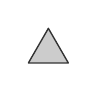
\begin{tikzpicture}[x=1in,y=1in,line cap=round,line join=round,sharp corners]
\fill[upfill] (0,0) -- (0.2,0) -- (0.1,0.1732) -- cycle;
\draw[iconline] (0,0) -- (0.2,0) -- (0.1,0.1732) -- cycle;
\end{tikzpicture}%
}}
\newcommand{\dn}{\raisebox{0.02em}{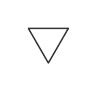
\begin{tikzpicture}[x=1in,y=1in,line cap=round,line join=round,sharp corners]
\fill[white] (0.1,0) -- (0,0.1732) -- (0.2,0.1732) -- cycle;
\draw[iconline] (0,0.1732) -- (0.1,0) -- (0.2,0.1732) -- cycle;
\end{tikzpicture}%
}}
\newcommand{\UP}{\textbf{UP}~\up}
\newcommand{\DOWN}{\textbf{DOWN}~\dn}

% ---- answer spaces ----
\newcommand{\ansbox}[1][0.6in]{\tikz[baseline=0in]\draw[line width=1.2pt,rounded corners=3pt] (0,-0.12in) rectangle (#1,0.38in);}
\newcommand{\blank}[1][1.2in]{\rule[-0.15em]{#1}{0.6pt}}
\newcommand{\writelines}[2][7.5in]{% #2 ruled lines, 0.34in apart
  \par\noindent\begin{tikzpicture}[x=1in,y=1in]
    \useasboundingbox (0,0.02) rectangle (#1,{-0.34*#2-0.04});
    \foreach \k in {1,...,#2}{\draw[line width=0.5pt,black!70] (0,-0.34*\k) -- (#1,-0.34*\k);}
  \end{tikzpicture}\par}

% ---- page header ----
\newcommand{\bandname}{}
\newcommand{\bandcolor}{pbblue}
\newcounter{sheet}
\newcommand{\sheethead}[1]{%
  \stepcounter{sheet}%
  \noindent
  \begin{tikzpicture}[x=1in,y=1in]
    \useasboundingbox (0,-0.62) rectangle (7.5,0.24);
    \node[anchor=west,font=\small,text=inkgray] at (0,0.08) {Bellingham Math Circle \,·\, Week 1: Tiling with pattern blocks};
    \node[anchor=east,font=\small\bfseries,text=white,fill=\bandcolor,rounded corners=6pt,inner sep=4pt] at (7.5,0.08) {\bandname};
    \draw[line width=0.6pt,draw=\bandcolor] (0,-0.08) -- (7.5,-0.08);
    \node[anchor=west,circle,fill=\bandcolor,text=white,font=\large\bfseries,inner sep=2pt,minimum size=0.36in] (n) at (0,-0.38) {\thesheet};
    \node[anchor=west,font=\LARGE\bfseries] at ($(n.east)+(0.08,0)$) {#1};
  \end{tikzpicture}\par\vspace{0.14in}}
\newcommand{\nameline}{\hfill{\large Name: \blank[2.2in]}\par\vspace{0.05in}}

% actual-size note with a 1-inch check bar
\newcommand{\actualsize}[1][Boards are actual size]{%
  \par\vfill\noindent
  {\footnotesize\color{inkgray}#1: each small triangle side is 1~inch. Print at 100\%.\hfill
   This bar is 1~inch:\,\tikz[baseline=-0.5ex]{\draw[line width=0.8pt] (0,-0.05in)--(0,0.05in) (0,0)--(1in,0) (1in,-0.05in)--(1in,0.05in);}}\par}

% boxes
\newcommand{\boxit}[3][\linewidth]{%
  \par\noindent\begin{tcolorbox}[width=#1,colback=\bandcolor!6,colframe=\bandcolor,boxrule=1pt,arc=6pt,
     left=5pt,right=5pt,top=4pt,bottom=4pt,boxsep=0pt,before skip=0pt,after skip=0pt]
     \raggedright\textbf{#2} #3
  \end{tcolorbox}\par}
\newcommand{\talk}[2][\linewidth]{\boxit[#1]{Talk about it.}{#2}}
\newcommand{\lab}[1]{\tikz[baseline=-0.6ex]\node[circle,draw=\bandcolor,line width=1.2pt,text=\bandcolor,font=\bfseries,inner sep=1.5pt,minimum size=0.3in]{#1};}

\renewcommand{\bandname}{Grades 4--5}
\renewcommand{\bandcolor}{pbblue}
\newcommand{\recgrid}[1]{\begin{tabular}{@{}c@{}}\fig{g45_tall_rec}\\[2pt]\textbf{#1}\end{tabular}}
\newcommand{\bigrec}{\fig{g45_big_rec}}

\begin{document}\large

% ===================================================== 1
\sheethead{Three blues, two ways}
\nameline
Today we only use \textbf{blue rhombi}. On our grid a blue can sit in three directions:

\vspace{0.08in}
\centerline{\fig{g45_dirs}}

\vspace{0.15in}
\noindent
\begin{minipage}[c]{2.3in}\fig{g45_hex1}\end{minipage}\hfill
\begin{minipage}[c]{4.9in}
\textbf{1.} Cover this hexagon with 3 blues.
There are exactly \textbf{two} ways. Build both.

\vspace{0.12in}
\textbf{2.} Lift the three blues and turn them, so that one way becomes the other.
This move is called a \textbf{flip}.
\end{minipage}

\vspace{0.1in}
\begin{center}\fig{g45_hex1_flip}\end{center}

\vspace{0.05in}
\textbf{3. Look in 3D.} Here are the same two tilings, shaded: one direction white,
one light gray, one dark gray. Stare at them. What do you see?
What does a flip do to the picture?

\vspace{0.05in}
\begin{center}\fig{g45_hex1_cubes}\end{center}
\writelines{2}

\vspace{0.12in}
\boxit{Coming up.}{Bigger hexagons have many tilings. You will hunt for all of them,
connect them by flips, and find a secret code hiding inside every tiling.}
\actualsize[Hexagon board is actual size]
\newpage

% ===================================================== 2
\sheethead{The tall hexagon}
\noindent
\begin{minipage}[t]{3.1in}\vspace{0pt}\fig{g45_tall}\end{minipage}\hfill
\begin{minipage}[t]{4.1in}\vspace{0pt}
Cover this board with 8 blue rhombi. This is called a \textbf{tiling}.

\vspace{0.12in}
How many \emph{different} tilings can your group find? Draw each new one in a box
below and give it a letter.

\vspace{0.12in}
\boxit{Tips.}{\begin{itemize}[leftmargin=1.1em]
\item One person builds, one checks that it is new, one draws.
\item Stuck? Look for three blues that make a small hexagon, and flip them!
\end{itemize}}
\end{minipage}

\vspace{0.2in}
\noindent
\recgrid{A}\hfill\recgrid{B}\hfill\recgrid{C}\hfill\recgrid{D}

\vspace{0.12in}
\noindent
\recgrid{E}\hfill\recgrid{F}\hfill\recgrid{G}\hfill\recgrid{H}

\vspace{0.12in}
We found \blank[0.6in] tilings. Are you sure there are no more? Why?
\writelines{2}
\actualsize[Big board is actual size]
\newpage

% ===================================================== 3
\sheethead{Flips}
\noindent
\begin{minipage}[c]{4.1in}\fig{g45_flip_example}\end{minipage}\hfill
\begin{minipage}[c]{3.2in}
Wherever three blues make a small hexagon (shaded yellow), you can flip them.
Two tilings are \textbf{neighbors} if one flip changes one into the other.
\end{minipage}

\vspace{0.2in}
\textbf{1. Flip map.} Write the letters of your tilings from page 2 in this box.
Draw a line between every pair of neighbors. Move letters around until your map looks tidy.

\vspace{0.08in}
\noindent\tikz{\draw[line width=1pt,rounded corners=6pt,draw=\bandcolor] (0,0) rectangle (7.45in,2.45in);}

\vspace{0.2in}
\noindent
\begin{minipage}[c]{1.6in}\centering\fig{g45_tall_LLRR}\\[2pt]\textbf{X}\end{minipage}
\begin{minipage}[c]{1.6in}\centering\fig{g45_tall_RRLL}\\[2pt]\textbf{Y}\end{minipage}\hfill
\begin{minipage}[c]{4.0in}
\textbf{2.} What is the fewest number of flips that turns X into Y?\quad\blank[0.5in]

\vspace{0.1in}
How do you know it can't be done in fewer?
\end{minipage}
\writelines{1}

\vspace{0.15in}
\textbf{3. Round trips.} Start at a tiling, make flips, and come back to where you started.
Count the flips. Can you find a round trip with an \emph{odd} number of flips?
\writelines{2}
\newpage

% ===================================================== 4
\sheethead{Ribbons: a secret code}
\noindent
\begin{minipage}[c]{2.75in}\fig{g45_ribbon_example}\end{minipage}\hfill
\begin{minipage}[c]{4.5in}
Start at the \textbf{top edge}. The blue touching it has a matching edge at its bottom.
The next blue shares that edge. Keep going down to the bottom edge.
This chain of blues is a \textbf{ribbon}.

\vspace{0.12in}
Each step of a ribbon goes down-left (\textbf{L}) or down-right (\textbf{R}).
The ribbon in the picture spells \textbf{L\,R\,R\,L}.
\end{minipage}

\vspace{0.2in}
\textbf{1.} Shade the ribbon in each of your tilings from page 2 and write its word.

\vspace{0.1in}
\begin{center}
\setlength{\extrarowheight}{6pt}
\begin{tabular}{|c|*{8}{>{\centering\arraybackslash}p{0.62in}|}}
\hline
\textbf{Tiling} & A & B & C & D & E & F & G & H \\\hline
\textbf{Word} & & & & & & & & \\[6pt]\hline
\end{tabular}
\end{center}

\vspace{0.1in}
\textbf{2.} List \emph{every} word made of two L's and two R's. Does each word give a tiling?
So how many tilings does the tall hexagon have?
\writelines{2}

\vspace{0.15in}
\textbf{3.} Pick two neighbors from your flip map and compare their words.
What does one flip do to the word?
\writelines{1}

\vspace{0.15in}
\textbf{4.} The \textbf{L-score} of a word is the sum of the places where the L's are.
For L\,R\,R\,L it is 1\,+\,4\,=\,5. What does one flip do to the L-score?
Use this to explain why a round trip can \emph{never} have an odd number of flips.
\writelines{3}
\newpage

% ===================================================== 5
\sheethead{The big hexagon}
\noindent
\begin{minipage}[t]{4.1in}\vspace{0pt}\fig{g45_big}\end{minipage}\hfill
\begin{minipage}[t]{3.1in}\vspace{0pt}
Tile this board with 12 blues. Now \textbf{two} ribbons start at the top edge.

\vspace{0.12in}
\centering\fig{g45_big_ribbons}\\[4pt]
{\normalsize Left ribbon: L\,R\,L\,R\\Right ribbon: R\,L\,R\,L}
\end{minipage}

\vspace{0.25in}
\textbf{1.} Build a tiling and find both ribbons.\\[4pt]
Left ribbon: \blank[1.1in]\qquad Right ribbon: \blank[1.1in]

\vspace{0.2in}
\textbf{2.} Can the two ribbons cross? Can they share a blue? Which pairs of words can
go together? (Your flip map from page 3 can help!)
\writelines{2}

\vspace{0.2in}
\noindent
\begin{minipage}[c]{4.95in}
\textbf{3. Challenge.} How many tilings does the big hexagon have?
Explain how you counted. Keep track on paper or a whiteboard.
\writelines[4.95in]{2}

\vspace{0.15in}
\textbf{4. Look in 3D.} Shade one of your tilings like the picture.
What do you see? What does a flip do to it?
\end{minipage}\hfill
\begin{minipage}[c]{2.25in}\raggedleft\fig{g45_big_cubes}\end{minipage}
\actualsize[Big board is actual size]
\end{document}
